\part{Implementierungsdetails}
Der Student hatte die Aufgabe im Rahmen seines Praktikums einen
``Gehaltsbenchmark für Mitteldeutschland`` im Bereich  Softwareentwicklung zu
konzeptionieren und umzusetzen. Ziel des Praktikums war der praktische Einatz
der neuen Software für das Unternehmen um dessen Produktpalette zu erweitern.
\section{statistische Berechnungen}
Um die erhaltenen Daten korrekt zu verarbeiten und zu berechnen wurden Formeln
aus der Statistik herangezogen. Folgende Berechnungen wurden für die Auswertung
der Daten getätigt:
\begin{itemize}
  \item Median \footnote{http://de.wikipedia.org/wiki/Median}
  \item Maximum \footnote{http://de.wikipedia.org/wiki/Gr\%C3\%B6\%C3\%9Ftes\_und\_kleinstes\_Element}
  \item Minimum \footnote{ebd.}
  \item Mittelwert \footnote{http://de.wikipedia.org/wiki/Mittelwert}
  \item oberes Quartil \footnote{http://de.wikipedia.org/wiki/Quartil}
  \item unteres Quartil \footnote{ebd.}
  \item Interquartilsabstand \footnote{ebd.}
  \item Ausreißerverdächtige Werte \footnote{http://de.wikipedia.org/wiki/Boxplot}
\end{itemize}
\section{Phasen der Implementierung}
Die Arbeit wurde in drei Phasen gegliedert. 
\begin{enumerate}
  \item Erweiterung des Webservices www.kanaleo.de um das Drupalmodul "Webform" 
  \item Verarbeitung und Bereitstellung der Daten mittels Ruby on Rails für die
Javascriptbibliothek Flotr2 
  \item Erstellung der Auswertung in Form eines PDFs, welches an den Kunden
ausgeliefert werden konnte
\end{enumerate}
\subsection{Erweiterung des Webservices www.kanaleo.de}
Zu Beginn der Arbeit wurde vom Autor in Zusammenarbeit mit dem Verantwortlichen
Herrn Dr. Jörg Klukas die Erweiterung des Webservices kanaleo.de
vereinbart. Dazu wurde nach einer gründlichen Recherche das Drupal-Modul
"Webform" für die Umsetzung des Projektes verwendet. Dieses Modul bot eine
schnelle Entwicklung des Fragebogens. Mittels eines vom Modul bereitgestellten
Baukastens konnten via ''Drag and Drop'' alle Elemente der Umfrage platziert
werden. Nachfolgend sehen Sie einen Auszug der Entwicklung des
Fragebogens.
\begin{figure}[htbp]
 \centering
 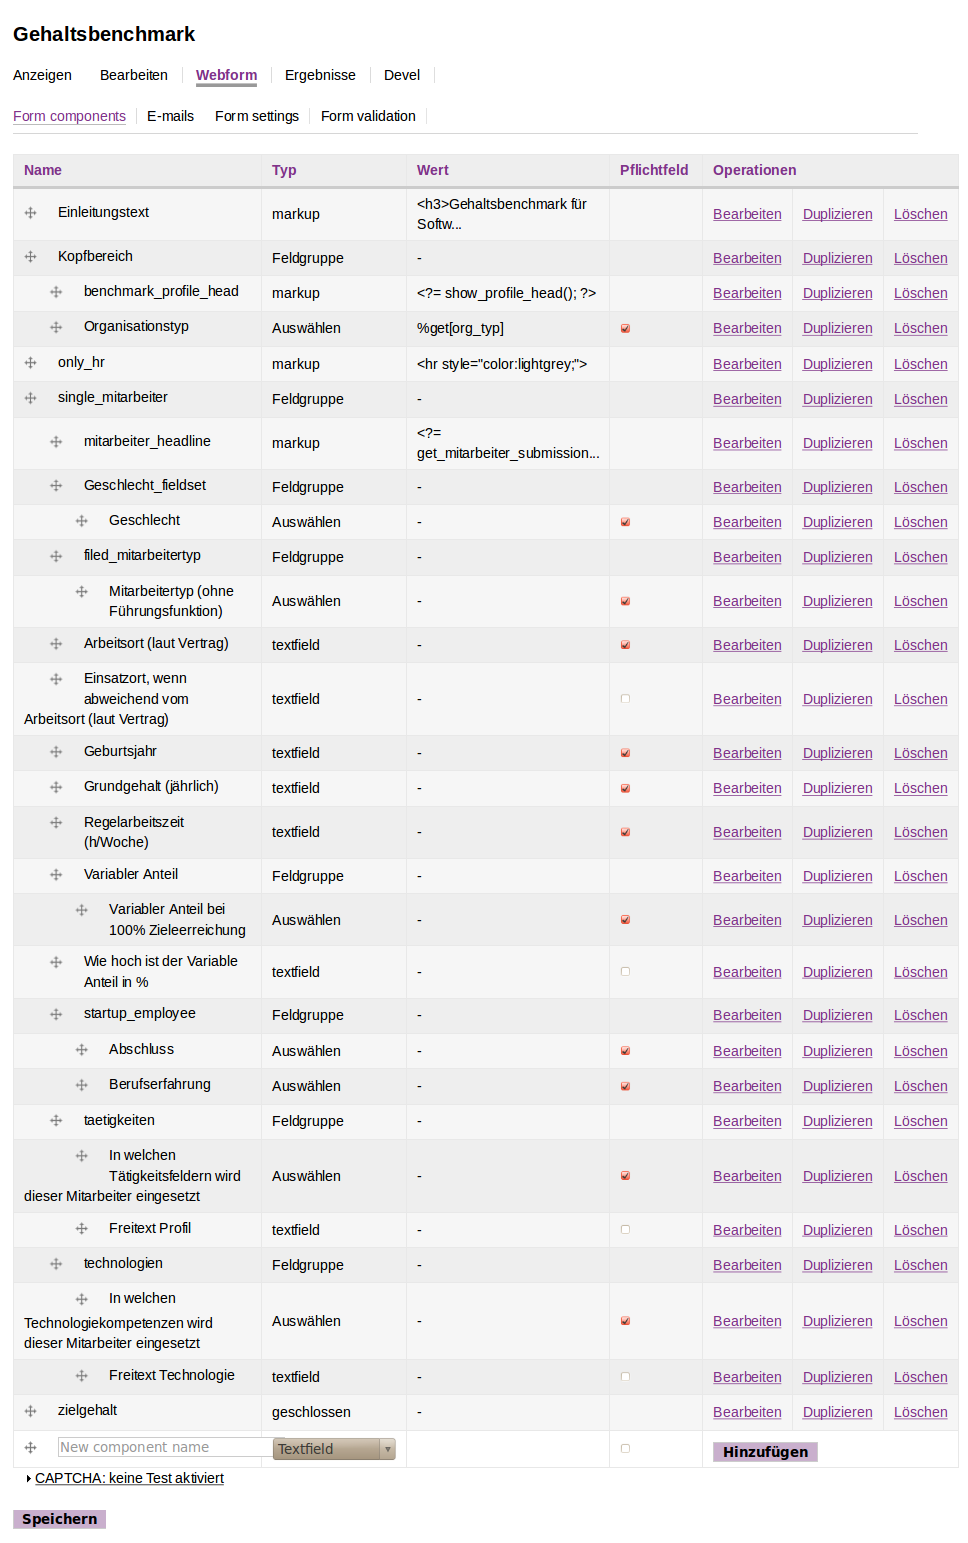
\includegraphics[width=350px]{./material/gehaltsformedit.png}
 % gehaltsformedit.png: 968x1543 pixel, 72dpi, 34.15x54.43 cm, bb=
 \caption{Auszug der Entwicklung des Fragebogens mittels des Moduls Webform}
 \label{fig: Fragebogen edit}
\end{figure}
\newpage
\subsection{Verarbeitung und Bereitstellung der Daten}
Die Wahl des Studenten fiel bei der Verarbeitung und Bereitstellung der Daten
auf das Framework Ruby on Rails. Der Grund hierfür war, dass das Praktikum
Möglichkeiten zum erlernen neuer Techniken einräumen sollte. Ruby, als Basis
des Frameworks, ist eine interessante Sprache, die dem Autor viel Raum zur
Umsetzung des Projektes gab. Anhand der nachfolgenden Auszüge des Programmcodes
wird der Student erläutern wie der Median zu berechnen war. \ref{lst:median}

\lstset{language=ruby}
\begin{lstlisting}[label=lst:median,caption=Auszug: Berechnung des Medians und des Durchschnitts]
class Array
  def median
    case self.size % 2 
    when 0 then self.sort[self.size/2-1,2].mean 
    when 1 then self.sort[self.size/2].to_f 
    end if self.size > 0            
  end

  def mean                                                                                                                                                   
    sum / count.to_f
  end 
end
\end{lstlisting}
Im obigen Quelltextausschnitt werden auf allen Arrays bzw. Listenobjekten die Methoden \texttt{median} und mean (Durchschnitt) angewendet. Die Berechnung erfolgt anhand der Vorschrift zur Berechnung des Medians\footnote{http://de.wikipedia.org/wiki/Median}.
Aufgerufen werden die Methoden dann als Objektmethoden jedes weiteren Array-Objektes, beispielhaft in Listing \ref{lst:mean}.
\begin{lstlisting}[label=lst:mean,caption=Beispiel des Durchschnitts und des Medians]
[1,2,5,10].mean # -> 4.5
[1,2,5,10].median # ->3.5
\end{lstlisting}
\newpage
\subsection{Erstellung der Auswertung in Form eines PDFs}
\label{sec:pdf_auswertung}
Die Auswertung wurde in drei Teile gegliedert. 
\begin{enumerate}
 \item die Stichprobenzusammensetzung,
 \item der allgemeine Teil, in dem alle abgegebenen Daten, aller Teilnehmer, ausgewertet werden,
 \item die personalisierte Auswertung.
\end{enumerate}
Das im
\fullref{sec:entwurf} erwähnte Bezahlmodell wird nachfolgend anhand von
Screenshots der Auswertung näher erläutert. 
\subsubsection{Stichprobenzusammensetzung}
In der Stichprobenzusammensetzung findet man einen Überblick über den Umfang der Daten. Diese werden in Torten- und Balkendiagrammen dargestellt. Alle Ergebnisse der Tortendiagramme sind Prozentangaben und die Balkendiagramme sind Absolutwerte.
\begin{figure}[htbp]
 \centering
 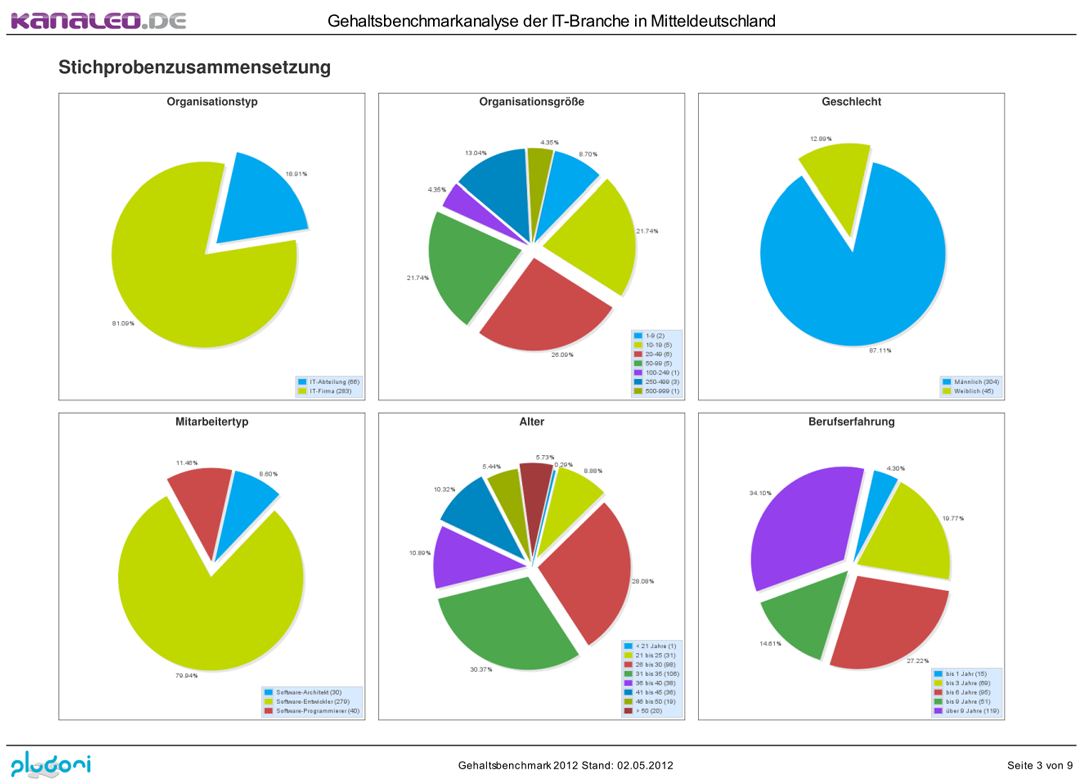
\includegraphics[width=350px]{./material/auszug_ueberblick_1.png}
 % auszug_ueberblick_1.png: 1080x779 pixel, 72dpi, 38.10x27.48 cm, bb=
 \caption{Auszug der Stichprobenzusammensetzung}
 \label{fig:Ueberblick_1}
\end{figure}
\begin{figure}[htbp]
 \centering
 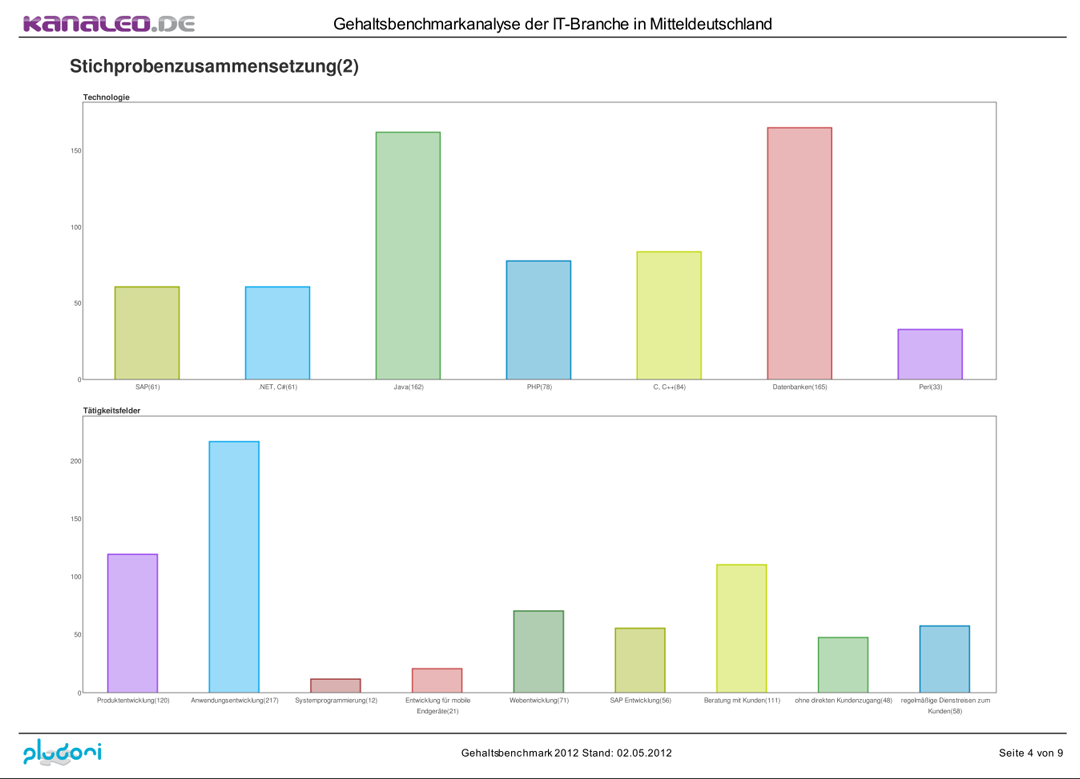
\includegraphics[width=350px]{./material/auszug_ueberblick_2.png}
 % auszug_ueberblick_1.png: 1080x779 pixel, 72dpi, 38.10x27.48 cm, bb=
 \caption{Auszug der Stichprobenzusammensetzung 2}
 \label{fig:Ueberblick_2}
\end{figure}
\subsubsection{Allgemeine Auswertung}
Der zweite Teil der Auswertung ist der allgemein, also eine Übersicht über alle Daten die abgegeben wurden. Dieser und der erste Teil sind für jeden unter bestimmten Voraussetzungen einsehbar. Entweder man möchte den Teil der Umfrage ohne Teilnahme, dann muss ein Betrag von 590€ gezahlt werden oder man möchte Teilnehmen und die Auswertung erhalten ohne Partner einer Empfehlungscommunity zu sein, dann muss ein Betrag von 990€ entrichtet werden. Im falle ein Teilnehmer ist Partner einer der Communitys ITsax.de oder ITmitte.de, dann ist die Teilnahme und der Erhalt der kompletten Auswertung kostenfrei.
\newpage
\begin{figure}[htbp]
 \centering
 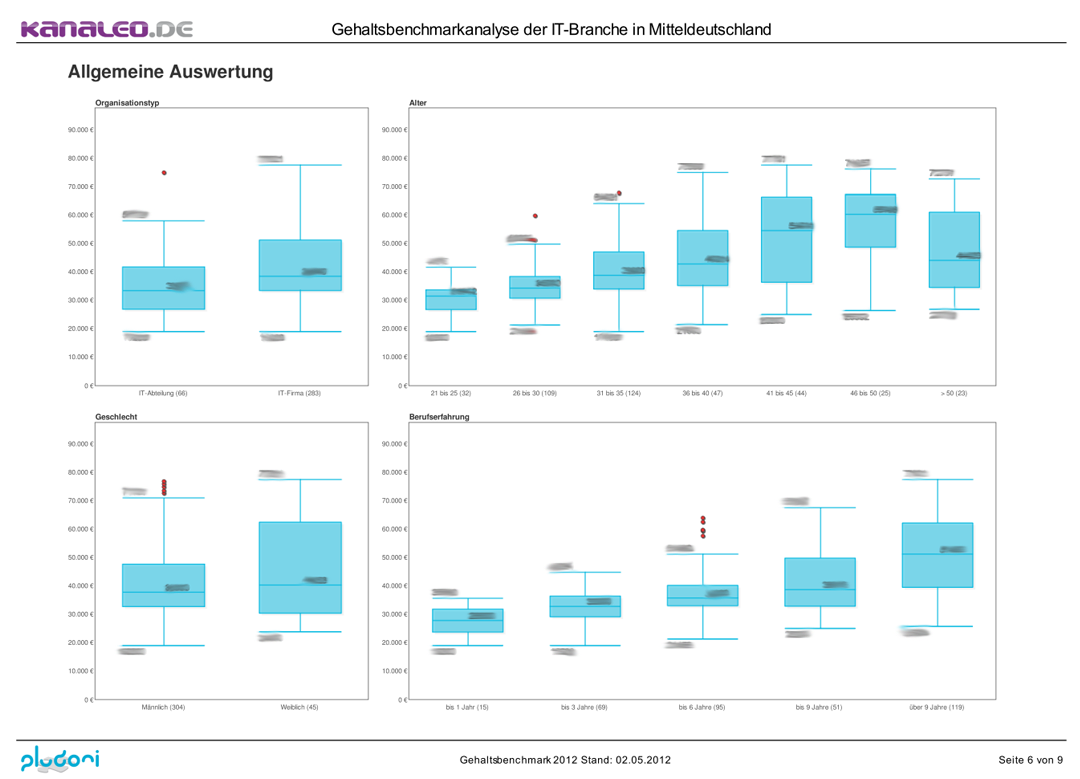
\includegraphics[width=350px]{./material/allgemeine_auswertung.png}
 % auszug_ueberblick_1.png: 1080x779 pixel, 72dpi, 38.10x27.48 cm, bb=
 \caption{Auszug der allgemeinen Auswertung}
 \label{fig:allg_auswertung}
\end{figure}
\subsubsection{Persönliche Auswertung}
Im dritten Teil geht es um den Teilnehmer persönlich. Das
heißt, die Daten des teilnehmenden Unternehmens werden ausgewertet und mit allen
anderen Werten verglichen. So erhält man eine gute Übersicht über die
Ergebnisse. Die Erstellung des PDFs erfolgte mittels
''wkhtmltopdf''\footnote{http://code.google.com/p/wkhtmltopdf/}. Dieses Tool
ist eine simple Shell-Anwendung, die es ermöglicht aus einem HTML-Dokument ein
PDF zu generieren. Dabei nutzt das Tool webkit\footnote{http://www.webkit.org/}
und qt\footnote{http://qt.nokia.com/products/}. 
\begin{figure}[htbp]
 \centering
 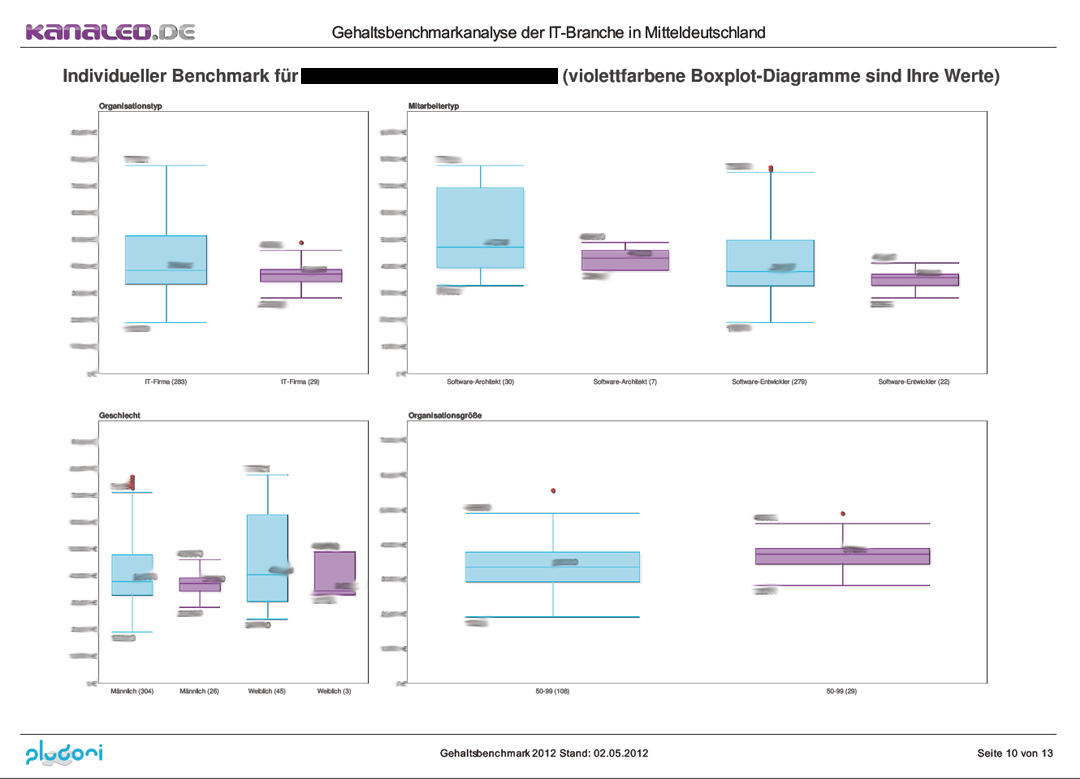
\includegraphics[width=350px]{./material/pers_auswertung.png}
 % auszug_ueberblick_1.png: 1080x779 pixel, 72dpi, 38.10x27.48 cm, bb=
 \caption{Auszug der persönlichen Auswertung}
 \label{fig:pers_auswertung}
\end{figure}
